\documentclass[11pt]{article}

% Change "review" to "final" for the camera-ready version,
% or to "preprint" for a non-anonymous version with page numbers.
\usepackage[review]{acl}

% Standard package includes
\usepackage{times}
\usepackage{latexsym}
\usepackage[T1]{fontenc}
\usepackage[utf8]{inputenc}
\usepackage{microtype}
\usepackage{inconsolata}
\usepackage{graphicx}

% ---- draft annotations: set \draftfalse to hide ----------------------
\usepackage{xcolor}
\newif\ifdraft
\drafttrue
\newcommand{\todo}[1]{\ifdraft\textcolor{red}{\textbf{[TODO: #1]}}\fi}

% ---- shorthands ------------------------------------------------------
\newcommand{\bench}{\textsc{UnpinBench}}
\newcommand{\dibench}{DI-Bench}
\newcommand{\code}[1]{\texttt{\small #1}}
% ---- every count in the paper is defined once, here --------------------
% screening population
\newcommand{\nCand}{622}        % candidates screened
\newcommand{\nRepos}{80}        % gold-passing repositories in the population
\newcommand{\nGold}{96}         % published solutions in the regular subset
\newcommand{\nGoldPass}{51}     % of which still pass
% dispositions
\newcommand{\nPairs}{330}       % verified pairs (the benchmark)
\newcommand{\nPoolRepos}{73}    % repositories with at least one pair
\newcommand{\nSilent}{226}      % CI passes without the package
\newcommand{\nExcl}{66}         % excluded with a stated reason
% decomposition of the silent cases
\newcommand{\nOverDecl}{173}
\newcommand{\nNoImport}{14}
\newcommand{\nStrict}{34}
\newcommand{\nOptional}{5}
% per-repository reporting
\newcommand{\nReposThree}{49}   % repositories with >= 3 candidates
\newcommand{\nIncidence}{33}    % of which have >= 1 silent candidate
\newcommand{\medianRate}{18.8}  % per-repository median, percent
\newcommand{\nSwirlCand}{165}   % the outlier repository's candidates
\newcommand{\nSwirlSilent}{126}
% tiers
\newcommand{\nTierNarrow}{196}
\newcommand{\nTierMedium}{41}
\newcommand{\nTierWide}{65}
\newcommand{\nTierIndirect}{28}
% grader validation
\newcommand{\nVariants}{617}    % all constructed variants
\newcommand{\nCounterfeit}{537} % counterfeit removals (seven kinds)
\newcommand{\nHonest}{80}       % honest deletions (control)
\newcommand{\nPseudo}{80}       % well-formed-but-incorrect rewrites
\newcommand{\nPseudoTraced}{15} % of which fall on a recorded pair
\newcommand{\nTracedPairs}{143}  % pairs with a recording
\newcommand{\nTraceInst}{172}    % recordings in total
\newcommand{\nTraceCalls}{68{,}942}   % published copy; 87,675 recorded
\newcommand{\nFuzzInputs}{300}  % generated inputs per function
% agent pilot
\newcommand{\nAgents}{4}
\newcommand{\nAgentTasks}{15}
\newcommand{\nAgentAttempts}{52}
\newcommand{\nAgentPass}{7}
% placeholders, to be filled when the hand-written removals are graded
\newcommand{\nRefs}{32}
\newcommand{\nRefsBehav}{\todo{k}}
\newcommand{\nStepOnly}{36}       % pairs admitted on a failing step with no import error
\newcommand{\nStepOnlyDirect}{13} % of which outside the indirect tier
% ---- added 10 Oct: measured in this pass (see docs/RESULTS_LEDGER.md)
\newcommand{\nStrictRepos}{21}
\newcommand{\nSilentConfirmed}{226}
\newcommand{\nSilentUnconfirmed}{13}
\newcommand{\nRefsPass}{32}
\newcommand{\nFRAccepted}{166}
\newcommand{\nFRInconclusive}{5}
\newcommand{\nCollectionSilent}{309}
\newcommand{\nImportSilent}{224}
\newcommand{\nScreened}{569}
\newcommand{\fidelityWhole}{89.9}
\newcommand{\nRefsEvaluable}{11}
\newcommand{\nRefsObservable}{5}
\newcommand{\nRefsObservableAccepted}{5}
\newcommand{\nRefsUnobservable}{6}
\newcommand{\nRefsUnobservableAccepted}{2}
% ---- activation rule applied (10 Oct, corrected reruns): 13 silent runs whose replay never announced the block are set aside (results/activation.json)
\newcommand{\nSilentAll}{239}        % before the rule
\newcommand{\nExclReason}{53}        % excluded with a construction reason
\newcommand{\nExclInconclusive}{13}  % excluded: block not observed loading
\newcommand{\medianRateAll}{20.0}
\newcommand{\nIncidenceAll}{35}
\newcommand{\nReposThreeAll}{51}
\newcommand{\dropTenMedian}{12.5}
\newcommand{\dropTenMedianAll}{14.3}
\newcommand{\nOverDeclGraded}{172}  % the over-declared set as graded (built before the recount)
\newcommand{\nFRFlagged}{1}
\newcommand{\nImportCatchesCIMisses}{34}
\newcommand{\nCIcatchesImportMisses}{32}
\newcommand{\nCollectionCatches}{247}
\newcommand{\nScreenedRule}{556}
\newcommand{\nPredSubset}{214}
\newcommand{\nPredSubsetSilent}{53}
\newcommand{\nMajorAffected}{10}
\newcommand{\nMajor}{12}
\newcommand{\nPseudoEvaluable}{6}
\newcommand{\nPseudoFunctions}{8}
\newcommand{\gThreeK}{16}          % tokens per hash
\newcommand{\gThreeW}{8}           % winnowing window
\newcommand{\gThreeThreshold}{60}  % containment threshold, percent
\newcommand{\gThreeMinTokens}{60}
\newcommand{\nVendorNamed}{67}
\newcommand{\nVendorNamedCaught}{67}
\newcommand{\nVendorRenamed}{20}
\newcommand{\nVendorRenamedCaught}{20}
\newcommand{\nVendorRepl}{52}      % replication corpus vendor variants
\newcommand{\nVendorReplCaught}{51} % the 52nd adds no Python file
\newcommand{\nRefsGThreeFlagged}{0}
\newcommand{\nPseudoGThreeFlagged}{0}
% ---- prose figures moved into macros (10 Oct, results pass)
\newcommand{\nGoldLarge}{50}
\newcommand{\nGoldLargeCompared}{45}
\newcommand{\nGoldLargePass}{29}
\newcommand{\nGoldFail}{45}
\newcommand{\dropTenIncidence}{23 of 39}
\newcommand{\corrTestShare}{-0.30}
\newcommand{\predPrecision}{0.62}
\newcommand{\predRecall}{0.79}
\newcommand{\predBaseRate}{0.25}
\newcommand{\predPrecisionAll}{0.80}
\newcommand{\predRecallAll}{0.88}
\newcommand{\closurePrecision}{0.34}
\newcommand{\closureRecall}{0.49}
\newcommand{\closureFlagged}{76}
\newcommand{\closureNoticed}{50}
\newcommand{\nStubSurvive}{15}
\newcommand{\nVendorSurvive}{19}
\newcommand{\nWeakenSurvive}{2}
\newcommand{\nRecLoadedNoCall}{117}
\newcommand{\nRecNotObserved}{6}
\newcommand{\nRecNotGreen}{64}
\newcommand{\nPseudoOutside}{65}
% ---- references through the two-level behavioural gate (results/references_g4.json, 10 Oct)
\newcommand{\nRefsAccepted}{5}
\newcommand{\nRefsInconclusive}{6}
\newcommand{\nRefsRejected}{0}
\newcommand{\nRefsNoCalls}{3}
\newcommand{\nRefsNotObservable}{3}
\newcommand{\nRefsNewModuleAccepted}{4}

% --- comparison fidelity and verdict stability (docs/COMPARISON_FIDELITY.md,
% --- docs/FLAKINESS.md). Both measured by re-running, not argued.
\newcommand{\fidelityRepr}{5.2}            % decided on a type and repr alone
\newcommand{\fidelityWholeBefore}{86.5}    % same projects, earlier summariser
\newcommand{\nRepeatCompared}{753}         % patch-matched pairs compared twice
\newcommand{\nRepeatFlips}{0}              % verdicts that differed
\newcommand{\nRepeatVerified}{330}         % verified pairs, red again
\newcommand{\nRepeatSilent}{226}           % silent pairs, green again
\newcommand{\nRepeatExcluded}{13}          % superseded by the blocker correction

% --- reference provenance (references/SUMMARY.md, references/UNWINNABLE.md)
\newcommand{\nRefsAttempted}{42}        % environment built, block verified live
\newcommand{\nRefsStrong}{25}
\newcommand{\nRefsMedium}{4}
\newcommand{\nRefsHard}{3}
\newcommand{\nRefsAbandoned}{10}        % solution exists in principle, not attempted
\newcommand{\nRefsRegular}{17}
\newcommand{\nRefsLarge}{15}
% --- agent sample (docs/AGENT_SAMPLE.md)
\newcommand{\nAgentSample}{100}
\newcommand{\nAgentSampleRepos}{71}
\newcommand{\nAgentSampleCapRepo}{4}
\newcommand{\nAgentSampleCapDep}{4}

% --- the GPT-5.1 agent run (docs/AGENT_RUN.md). Supersedes the 4-model pilot
% --- for the headline agent numbers; the pilot stays as the multi-model point.
\newcommand{\nAgentRunModel}{GPT-5.1}
\newcommand{\nAgentRunN}{100}
\newcommand{\nAgentRunCost}{10.17}
\newcommand{\nAgentRunPass}{19}
\newcommand{\nAgentRunPassNoIndirect}{15}
\newcommand{\nAgentRunNoIndirect}{91}
\newcommand{\nAgentRunAccepted}{1}
\newcommand{\nAgentRunRejected}{7}
\newcommand{\nAgentRunInconclusive}{11}
\newcommand{\nAgentRunUnstated}{2}
\newcommand{\nAgentRunFinish}{98}
\newcommand{\nAgentRunTouchTests}{30}
\newcommand{\nAgentRunGFourUnverified}{18}
\newcommand{\nAgentNarrowPass}{13}
\newcommand{\nAgentNarrowN}{60}
\newcommand{\nAgentMediumPass}{1}
\newcommand{\nAgentMediumN}{12}
\newcommand{\nAgentWidePass}{1}
\newcommand{\nAgentWideN}{19}
\newcommand{\nAgentIndirectPass}{4}
\newcommand{\nAgentIndirectN}{9}
% ---- replication corpus through the behavioural gates (results/g4_cheats.json, 10 Oct)
\newcommand{\nCheatCIPass}{61}        % hide 35, stub 8, vendor 18
\newcommand{\nCheatGFourEvaluable}{14}   % CI-passing variants G4a could speak for
\newcommand{\nStubCIPass}{8}
\newcommand{\nStubGFourEvaluable}{3}
\newcommand{\nStubGFourRejected}{1}
\newcommand{\nCheatNotRunnable}{47}   % of the 61: suite not runnable locally 34, jax/torch 11, no call 2
% ---- agent pilot through the grader (results/agent_grader.json, 10 Oct)
\newcommand{\nAgentAccepted}{1}      % humanlayer/python_slugify (DeepSeek): identical at the usage sites
\newcommand{\nAgentRejected}{2}      % openant/pyusb, omniduct/progressbar2: the declaration was never removed (G1; G8, G5 follow)
\newcommand{\nAgentInconclusive}{4}  % behavioural gate could not observe the replacement
\newcommand{\nAgentUnstated}{0}      % rejections resting only on a constraint the prompt did not state (trade, vendor)
\newcommand{\nRecNotObservedOld}{168}  % recorder never loaded, before the saved-fd fix
\newcommand{\nTracedPairsOld}{85}
\newcommand{\nTraceCallsRecorded}{87{,}675}  % before one trace was capped per site for publication
\newcommand{\nPseudoCannotSpeak}{5}   % on a traced pair, no evaluable function (opaque arguments, import name, hostile import)

% --- reading all 19 CI passes by hand (docs/AGENT_INSPECTION.md); partitions 19
\newcommand{\nInspCorrect}{3}
\newcommand{\nInspTrivial}{1}
\newcommand{\nInspUnverifiable}{4}
\newcommand{\nInspNotEquivalent}{4}
\newcommand{\nInspRejected}{7}
\newcommand{\nInspNeverRemoved}{3}
\newcommand{\nInspStillArrives}{4}

\usepackage{tikz}
\usetikzlibrary{arrows.meta,positioning}
\usepackage{pgfplots}
\pgfplotsset{compat=1.18}

\title{Remove This Dependency: Why Passing Tests Cannot Tell You\\
a Dependency Is Gone}

\author{First Author \\
  Affiliation / Address line 1 \\
  Affiliation / Address line 2 \\
  \texttt{email@domain} \\\And
  Second Author \\
  Affiliation / Address line 1 \\
  Affiliation / Address line 2 \\
  \texttt{email@domain} \\}

\begin{document}
\maketitle

\begin{abstract}
Execution-based benchmarks judge a repository-level change by whether the project's test suite still passes.
\dibench{} \citep{dibench2025} states the premise directly---``whether the tests pass is the most direct and reliable indicator of the correctness of the generated dependencies''---and its own limitations section raises test incompleteness only to set it aside.
We measure what that assumption costs.
Screening every dependency declared by every gold-passing repository in \dibench's Python subsets (622 candidates over 80 repositories), removing each declaration and making the package genuinely unimportable from the repository's own frames, we find the oracle stays silent in 226 cases.
That number decomposes, and the decomposition matters more than the total: 149 are over-declarations with no trace of the package anywhere, 23 are used without being imported, 8 are optional by design, and \textbf{46 are oracle blindness in the strict sense}---the code imports the package on a path no test exercises.
The rate is not uniform: a single repository declaring 172 dependencies supplies 126 of the 226, so we report the per-repository median (18.8\%) and the incidence (35 of 51 repositories have at least one) rather than a pooled figure.
The surviving 348 verified pairs form \bench, a benchmark for removing a dependency the code actually uses.
Because a passing suite also accepts several ways of faking a removal, we pair it with a gate stack and validate against 617 constructed cheats spanning eight families.
Each family is caught by its intended gate---but one is not: 80 of 80 \emph{pseudo-genuine} replacements, structurally indistinguishable from a real rewrite, survive every structural check.
That family motivates a behavioural gate, which is possible here and nowhere else: in a removal task the removed library is a canonical oracle, present and recordable before it is taken away.
\end{abstract}

\section{Introduction}
\label{sec:intro}

Every software project depends on libraries it does not maintain.
The packages a project declares change as code is written, refactored, and retired.
Keeping those declarations accurate, by adding what the code needs and removing what it no longer uses, is a recurring maintenance cost \citep{mcintosh2011build}, and the declared packages determine a project's install size and its exposure to vulnerabilities \citep{drosos2024bloat}.
Language-model agents are increasingly assigned this work, and benchmarks measure their progress.
A benchmark can do so only if its tasks are real and solvable and its grader returns a verdict that can be trusted.

Benchmarks for dependency tasks follow the pattern established by SWE-bench \citep{jimenez2024swebench}: a real repository, a task, and a grader that executes the project's own code.
\dibench{} \citep{dibench2025} masks a repository's declarations and asks a model to restore them.
EnvBench \citep{envbench2025} and Repo2Run \citep{repo2run2025} ask an agent to make a repository build and run.
Their tasks differ, but their graders differ only in what they check: the full CI workflow, a type checker's import resolution, or test collection alone.
All of them treat a passing check as evidence that the dependency set is correct.

However, execution-based grading is not self-validating.
An audit of ten widely used agentic benchmarks found outcome-validity flaws in seven \citep{abc2025}, and on SWE-bench, 29.6\% of patches that pass the tests behave differently from the developer's fix \citep{patchdiff2026}.
For dependency tasks the oracle can fail in two distinct ways.
The first is blindness. A test suite can detect that a package is absent only if some test executes the code that imports it, and only if the import fails when executed.
Benchmark authors acknowledge that coverage is incomplete, but how often this assumption fails has not been measured.
The second is the counterfeit removal, which arises exactly where the tests are not blind.
Where the suite would catch a naive removal, passing it still does not show that a removal happened: moving the declaration to another section, vendoring the library, stubbing it with well-formed but incorrect values, or weakening a test can all pass.
Blindness has to be measured, so that tasks are built only where the oracle can see.
Counterfeits have to be caught, which needs a check the test suite does not provide.

One dependency task is absent from this landscape, and it is the task for which a better oracle exists.
Inference benchmarks restore declarations, debloating tools \citep{pytrim2025,soto2021longitudinal} remove declarations the code no longer uses, and migration benchmarks \citep{pymigbench2023} replace one library with another.
No benchmark evaluates removing a dependency that the code actually uses, which requires rewriting the code so that the library is no longer needed.
Maintainers do this when a library is abandoned, vulnerable, or far larger than the function it provides.
The task has a property that migration tasks share but no benchmark has used.
A test suite is an oracle by sampling: it checks the behaviours its authors thought to check.
The library being removed is an oracle by construction: it is a correct implementation of exactly the behaviour a replacement must preserve, and it is present and recordable before it is taken away.
Program repair must compare a candidate patch against a human patch that may itself be wrong \citep{ye2021rgt,patchdiff2026}, and test-strengthening methods must synthesise tests whose intent is uncertain \citep{sting2026}.
A removal task supplies its own reference, and our grader is built on it.
The reference is not complete: the library supplies the expected outputs, but the tests still supply the inputs, so we extend the recorded inputs with generated neighbours.

We measure the blindness, build a benchmark where the oracle can see, and build a grader on the library.
We screen \nCand{} candidates: every dependency declared by the \nRepos{} \dibench{} Python repositories whose published solution still passes.
For each, we delete the declaration, make the package unimportable from the repository's own code, and rerun its CI workflow.
The tests pass without the package for \nSilent{} candidates, and a further \nExclInconclusive{} pass in runs where the block cannot be shown to have loaded, which we set aside.
Most of the \nSilent{} are declarations the code never uses; in \nStrict, the code imports the package on a path no test reaches, which is oracle blindness in the strict sense.
In the median repository among the \nReposThree{} with at least three candidates, the tests are indifferent to one declared dependency in five: keeping it and omitting it both pass.
\nIncidence{} of the \nReposThree{} have at least one such dependency.
An inference grader therefore cannot tell whether these declarations were restored, and for the \nStrict{} it accepts an omission that breaks code no test runs.
The \nPairs{} candidates whose removal fails CI because of the repository's own use of the package form \bench, over \nPoolRepos{} repositories, of which \nTierIndirect{} form an indirect track reached through a tool or plugin rather than an import; the disposition of every candidate is published.
\nRefsPass{} of \nRefs{} hand-written removals pass the workflow with the package blocked, so the task is solvable where it was tried.

We then construct \nVariants{} variants, \nCounterfeit{} counterfeit removals of seven kinds and \nHonest{} honest deletions that must pass, and grade them with seven checks, which we call gates, one of which is the test suite itself.
The structural gates alone reject 72\% to 100\% of each of six kinds and none of the seventh: a replacement with the form of a genuine rewrite that returns incorrect values.
The behavioural gate records the library during the project's own tests and compares the replacement against the record.
It can speak only where a recording exists, which is currently \nTracedPairs{} of the \nPairs{} pairs.
Only \nPseudoTraced{} of the \nPseudo{} counterfeit rewrites fall on such a pair; the gate could evaluate four of them, five functions in all, and it rejects every one.
Where it cannot speak, the grader does not return a pass: it reports the structural verdict and marks the behavioural one as inconclusive.
Of \nOverDeclGraded{} removals that are correct by construction, the candidates the code never uses, the grader accepts \nFRAccepted, cannot resolve the dependency closure of \nFRInconclusive, and flags \nFRFlagged{} that was not in fact a removal.
Of the \nRefsEvaluable{} hand-written rewrites whose suites call the library locally, the behavioural gate accepts \nRefsAccepted, returns inconclusive on \nRefsInconclusive{} it cannot observe, and rejects none; where it cannot see, it says so rather than guessing.
In a pilot of \nAgents{} coding agents on \nAgentTasks{} tasks, \nAgentPass{} of \nAgentAttempts{} attempts pass the test suite, the number a conventional benchmark would report.
Of those \nAgentPass, the grader rejects \nAgentRejected{} and leaves the behavioural verdict inconclusive for \nAgentInconclusive{}.

\paragraph{Contributions.}
\begin{itemize}
\item A census of the test oracle on dependency removal, with every silent case attributed to one of four causes (\S\ref{sec:rq1}).
\item \bench: \nPairs{} removal pairs over \nPoolRepos{} repositories, published with the disposition of every screened candidate and with hand-written reference removals for \nRefs{} of them (\S\ref{sec:construction}).
\item A seven-gate grader that retains the tests as one gate, validated on \nCounterfeit{} counterfeit removals of seven kinds and \nHonest{} honest deletions as a control (\S\ref{sec:gates}).
\item The grader's behavioural gate, which uses the removed library as the oracle: the only gate that rejects a well-formed but incorrect rewrite, with its coverage and the boundary of its false rejection measured (\S\ref{sec:behaviour}).
\end{itemize}

\section{Background and Related Work}
\label{sec:related}

\paragraph{Dependency inference and its oracle.}
\dibench{} \citep{dibench2025} is the closest benchmark to our setting: 581 repositories across four languages, dependency declarations masked, and both textual metrics (precision and recall over package names) and an execution metric.
Its authors note that ``test coverage for each repository may not be exhaustive'' and leave the consequence unexplored.
We quantify that consequence.
DependEval \citep{dependeval2025} evaluates repository dependency \emph{understanding} through static tasks and does not execute.
Environment-setup benchmarks \citep{envbench2025,repo2run2025} ask an agent to make a repository runnable at all, a different task with the same oracle and, we expect, the same blindness.

\paragraph{Tests as an oracle.}
That test suites miss dependency-induced faults is known.
\citet{hejderup2022trust} seeded faults into library call sites in Java projects and found test suites detected a minority.
More recently, \citet{timemachine2026} report agents producing ``spurious solutions that exploit low test coverage'' on dependency upgrades, and \citet{sweatlas2026} measure a 15--40 point gap between passing behavioural checks and meeting maintainability rubrics on refactoring tasks.
Our contribution is to mutate the \emph{manifest} rather than the code, which isolates the dependency oracle specifically, and to separate phantom installation from genuine test blindness.

\paragraph{Dependency bloat and debloating.}
A substantial literature detects and removes \emph{unused} dependencies: DepClean \citep{soto2021longitudinal} for Maven, PyTrim \citep{pytrim2025} for Python, and the fine-grained PyPI analysis of \citet{drosos2024bloat}.
These tools solve the easy case, where no code calls the library.
\bench{} targets the hard case, where the library is in use and removal requires writing a replacement.

\paragraph{Removal and migration datasets.}
\citet{he2021migration} mined 19,652 Java projects and found 8,065 with at least one library removal; a 2024 dataset of dependency-removal commits and their pull requests is publicly available \citep{jaisri2024dataset}.
Both are \emph{mined metadata}: they record that removals happened, but cannot score a candidate removal, because they carry no executable environment.
Library \emph{migration} benchmarks \citep{pymigbench2023,migrationbench2025} cover replacing library $A$ with library $B$, not eliminating a library in favour of one's own code.
LibReuseBench \citep{libreuse2026} and Commit0 \citep{commit02024} ask models to write code that avoids or reimplements libraries, but on greenfield problems with no existing code whose behaviour must be preserved.
To our knowledge no executable benchmark exists for in-situ removal of a used dependency.

\paragraph{Agent scaffolds and reward hacking.}
Our agent scaffold follows the agent-computer interface of SWE-agent \citep{sweagent2024}: a line-numbered viewer with a 100-line window, search results capped at 50, a range-based edit command with an integrated syntax linter, and collapsing of observations older than the last five.
Evaluation uses greedy decoding at temperature 0 with a single attempt, the standard \textit{pass@1} protocol.
That agents exploit weak verifiers is well documented.
\citet{specbench2026} separate visible from held-out tests and find most of the gap arises from compositional failure rather than deliberate cheating; \citet{hackerfixer2026} found 16\% of tasks across five agent benchmarks hackable from the task description alone.
We do not claim to measure reward hacking in general.
We claim something narrower and testable: on one concrete task, we enumerate the ways a change can pass the test oracle without doing the work, and we measure which gates catch which.

\section{Screening the Oracle and Building the Benchmark}
\label{sec:method-bench}

Figure~\ref{fig:pipeline} shows the method in two halves.
The first takes every declared dependency of a population of repositories, perturbs it, and records what the test oracle does: the dependencies the oracle detects become the benchmark, and those it misses become the census of its blindness.
The second records the library before it is removed and grades a submission against that record.
Five terms are used throughout: a \emph{candidate} is one declared dependency of one repository under screening; a \emph{pair}, a repository and one of its dependencies, is a candidate admitted as a task; a \emph{submission} is a change that claims to remove a pair's dependency; a \emph{removal} is the act of making a repository no longer need a library, or the change that does so; and a \emph{variant} is a submission we construct ourselves, counterfeit or honest.

\begin{figure*}[t]
\centering
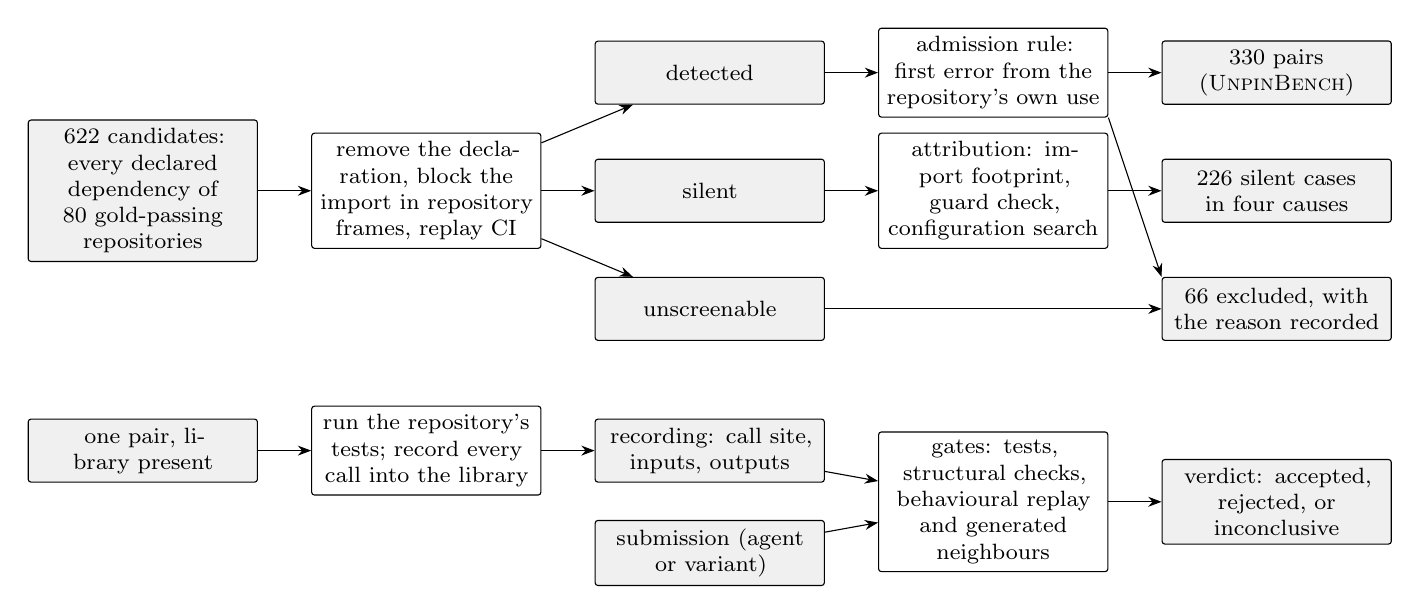
\begin{tikzpicture}[
  font=\footnotesize, >=Stealth,
  box/.style={draw, rounded corners=1pt, align=center, inner sep=3pt, text width=2.7cm, minimum height=8mm},
  data/.style={box, fill=black!6},
  proc/.style={box, fill=white}]
% ---- screening half
\node[data] (cand) at (0,0) {\nCand{} candidates: every declared dependency of \nRepos{} gold-passing repositories};
\node[proc] (screen) at (3.6,0) {remove the declaration, block the import in repository frames, replay CI};
\node[data] (det) at (7.2,1.5) {detected};
\node[data] (sil) at (7.2,0) {silent};
\node[data] (uns) at (7.2,-1.5) {unscreenable};
\node[proc] (admit) at (10.8,1.5) {admission rule: first error from the repository's own use};
\node[proc] (attr) at (10.8,0) {attribution: import footprint, guard check, configuration search};
\node[data] (pool) at (14.4,1.5) {\nPairs{} pairs (\bench)};
\node[data] (causes) at (14.4,0) {\nSilent{} silent cases in four causes};
\node[data] (excl) at (14.4,-1.5) {\nExcl{} excluded, with the reason recorded};
\draw[->] (cand) -- (screen);
\draw[->] (screen) -- (det); \draw[->] (screen) -- (sil); \draw[->] (screen) -- (uns);
\draw[->] (det) -- (admit); \draw[->] (sil) -- (attr);
\draw[->] (admit) -- (pool); \draw[->] (attr) -- (causes);
\draw[->] (admit.south east) -- (excl.north west); \draw[->] (uns) -- (excl);
% ---- grading half
\node[data] (pair) at (0,-3.3) {one pair, library present};
\node[proc] (rec) at (3.6,-3.3) {run the repository's tests; record every call into the library};
\node[data] (trace) at (7.2,-3.3) {recording: call site, inputs, outputs};
\node[data] (sub) at (7.2,-4.6) {submission (agent or variant)};
\node[proc] (gates) at (10.8,-3.95) {gates: tests, structural checks, behavioural replay and generated neighbours};
\node[data] (verdict) at (14.4,-3.95) {verdict: accepted, rejected, or inconclusive};
\draw[->] (pair) -- (rec); \draw[->] (rec) -- (trace);
\draw[->] (trace) -- (gates); \draw[->] (sub) -- (gates);
\draw[->] (gates) -- (verdict);
\end{tikzpicture}
\caption{Method overview. Top: every candidate is perturbed once and ends as a pair, a silent case attributed to one of four causes, or an exclusion with a stated reason (\S\ref{sec:method-bench}). Bottom: for each pair the library is recorded during the repository's own tests before it is removed, and a submission is graded against the tests, the structural gates, and that recording (\S\ref{sec:method-grade}).}
\label{fig:pipeline}
\end{figure*}

\subsection{Population and Harness}
\label{sec:setup}

\paragraph{Population.}
We use the two Python subsets of \dibench{}.
Each instance supplies a repository at a fixed commit, its dependency manifests, a published solution that we call the \emph{gold} manifest, and a command that replays the repository's own GitHub Actions workflow.
A repository enters the population only if its gold manifest passes that workflow in our harness.
The rule removes repositories whose suites fail for reasons unrelated to any dependency, so that a failure after a perturbation is attributable to the perturbation.
The population is \nRepos{} repositories, which together declare \nCand{} candidates.

\paragraph{Harness.}
Each replay runs inside a container on hosted GitHub Actions runners (Appendix~\ref{app:harness}).
The workflow is the repository's own, run as written: package installation has network access, and repository secrets are absent, so a step that needs one fails in the gold run and the repository does not enter the population.
Package versions are not pinned by us; they resolve at run time, so each run records its date and its resolved environment, and a verdict is a statement about the ecosystem on that date.
A job that never starts is counted as a failure rather than a pass, because the replay tool reports success for such a job, and under perturbation this is conservative for the census.
Such a candidate carries no attributable evidence and is excluded (\S\ref{sec:construction}).
The harness is otherwise \dibench's, and the changes we made to it are released.

\paragraph{Stability of a verdict.}
A verdict is the outcome of one replay, pass or fail.
To measure whether a verdict is stable we replay every candidate a second time with an identical manifest change and count the candidates whose verdict differs.
A pair that flips is not attributable to the dependency and leaves the pool; a silent case that flips is not blindness and leaves the census; a gold run that flips marks the repository as unstable, and all of its candidates leave with it.
\S\ref{sec:results} reports the counts.

\paragraph{Running example.}
\code{wikitextparser}, a parser for MediaWiki markup, declares \code{wcwidth}, a library that reports how many terminal columns a string occupies.
The repository imports it in one source file and calls it at two sites, and no test file imports it.
It belongs to the narrow tier (\S\ref{sec:construction}), which holds most pairs; the example is chosen for legibility, not for difficulty, and it is followed through each step below.

\subsection{Screening the Oracle}
\label{sec:screening}

\paragraph{Perturbation.}
For each candidate we edit the gold manifest so that the dependency is no longer declared, change nothing else, and replay the workflow.
Deleting the declaration alone does not remove the package from the environment, because another dependency may install it, so the perturbation also blocks the import.
The block is a module finder injected into the repository at its root, which refuses to import the removed package when the importing frame belongs to the repository's own code or tests and lets every other package import it freely (Appendix~\ref{app:harness}).
The scope matters: a third-party package that imports the removed library proves nothing about the repository, and a block that fired for every frame would blame repositories for failures that are not theirs.
What the block cannot see is a repository that runs from an installed copy of itself: frames are attributed by file path, so if the workflow installs the package non-editably and imports it from the environment, every frame reads as foreign and the block never fires.
The activation rule below exists for this case.

\paragraph{Outcomes.}
A candidate ends in one of three states.
It is \emph{detected} if the workflow fails.
It is \emph{silent} if the workflow passes.
It is \emph{unscreenable} if the distribution's import name is also the name of a standard-library module, because blocking that name would sever the standard library, and such candidates are excluded with that reason.
The block announces itself in the log when it loads, at interpreter start or inside the test runner, and a detected pair whose first error the block raised from a repository frame shows that the workflow attributes frames to the working tree.
A silent verdict is counted only when its log carries the announcement, or the package is never imported by the repository, in which case nothing could have triggered the block and its activation is immaterial; that the same repository has a detected pair raised from a repository frame is reported as corroboration but does not count on its own.
A silent run that meets neither condition is replayed, and excluded as inconclusive if it still meets neither.
For the running example the block raises at the import of \code{wcwidth}, from a frame in the repository's source file, and the workflow fails: the candidate is detected.

\paragraph{Attribution of silent cases.}
A silent verdict means the oracle did not notice the removal; it does not by itself mean the oracle was blind, because the declaration may have been wrong to begin with.
We attribute every silent case to one of four causes from three signals.
The \emph{import footprint} lists the repository's source files that import the package, from its abstract syntax trees.
The \emph{guard check} marks each such import that sits inside a handler for \code{ImportError} or \code{ModuleNotFoundError}.
The \emph{configuration search} looks for the package name, and its spelling variants, in packaging configuration, test-runner configuration, and workflow files.
The mapping is mechanical.
No footprint and no configuration mention: \emph{over-declared}, the declaration was unneeded.
No footprint but a configuration mention: \emph{used without importing}, a plugin, an entry point, a build backend, or a tool the workflow invokes.
A footprint in which every import is guarded: \emph{optional by design}, the code is written to run without the package.
A footprint with at least one unguarded import: \emph{oracle blindness in the strict sense}, the code needs the package on some path and no test reaches it.
The syntactic guard check does not test that a fallback works, which makes strict blindness a lower bound; the generous configuration search makes over-declaration a lower bound and use without importing an upper bound.
An unguarded import on an unreached path may sit in code that no user runs either; we do not distinguish such code from live code, and \S\ref{sec:limitations} returns to this.

\paragraph{Reporting rule.}
Candidates are not spread evenly across repositories; one repository declares \nSwirlCand{} of them.
A pooled rate would therefore measure that repository rather than the population.
We report the \emph{silent rate}: the share of a repository's candidates that are silent for any cause.
Over repositories with at least three candidates we give its median and its \emph{incidence}, the share with at least one silent candidate; the pooled rate is given only alongside these.
\emph{Blindness} is reserved for the strict cause.

\subsection{Constructing the Benchmark}
\label{sec:construction}

\paragraph{Admission.}
A detected candidate becomes a pair only if the failure arises from the repository's own use of the package.
The first error in the log must be one of four kinds: the block raised from a frame in the repository's code or tests; a missing-module error for the package raised from such a frame; a test failure with no import error anywhere, in a suite that passed with the package present; or a linter step that names the package.
The third and fourth kinds exist because a removal can surface without an import error, when the package was reached through a plugin or a tool rather than an import.
The third kind is the weakest, because a third-party package can change behaviour when its own optional dependency disappears; \nStepOnly{} pairs rest on it alone, \nStepOnlyDirect{} of them outside the indirect track, and each was read by hand before admission. % CONFIRM: hand check of all 36 under the current pool
A detected candidate whose first error is none of the four is excluded.
For the running example the evidence is the first kind, the block raised at the import in the repository's source file.

\paragraph{Exclusion.}
Scoping the block does not make every detected candidate admissible, because the perturbation changes two things: the block controls what an import does, and the deletion also changes what is installed.
A third-party package that silently relied on the repository's declaration fails on its own when the package is gone, and that failure is not the repository's.
Each exclusion carries one reason:
\begin{itemize}\setlength{\itemsep}{0pt}
\item the first error is raised inside another package, or from a frame that cannot be attributed, so the failure is not the repository's;
\item the removal exposed a second, undeclared package that the removed one had been supplying, so the failure concerns a different package;
\item every import of the dependency is guarded and the first error is not the repository's, so there is no removal to perform (\todo{n} candidates); % CONFIRM: the 7 optional-by-design exclusions have a non-repository first error; any with a repository test failure is a broken fallback and belongs in the pool
\item the workflow installs from a second source that also declares the package, so editing the manifest removes nothing;
\item the install step itself fails, so no test ran.
\end{itemize}
The excluded candidates are released with their reasons, alongside the pairs.

\paragraph{Tiers.}
Pairs are tiered by footprint, the number of source files that import the package.
\emph{Narrow} is one or two files, \emph{medium} three or four, and \emph{wide} five or more.
The tier describes how much of the repository a removal must touch; it is not a measured difficulty.
Pairs with no importing file, where the package is reached through a plugin, an entry point, or a tool the workflow invokes, form a separate \emph{indirect} track of \nTierIndirect{} pairs, counted within the \nPairs{}.
They are admitted on the third and fourth kinds of evidence, their removal eliminates the tool's use rather than rewriting call sites, and the solvability and false-rejection claims below do not cover them. % DECIDE: whether any reference covers the indirect track

\paragraph{Reference removals.}
Admission establishes that the oracle sees the removal; it does not establish that the removal can be done.
For \nRefs{} pairs we wrote the removal by hand: the declaration deleted, the code rewritten so that the library is no longer needed, and no new package added.
Pairs were taken in pool order from the tractable candidates rather than chosen for the gates, and the resulting spread follows the pool's: \nRefsStrong{} narrow, \nRefsMedium{} medium and \nRefsHard{} wide, \nRefsRegular{} regular and \nRefsLarge{} large.
Of \nRefsAttempted{} pairs attempted, \nRefs{} were completed and \nRefsAbandoned{} were set aside with a written reason, published with the references; the commonest reason is that a faithful replacement would be a wire-protocol implementation of several hundred lines, which is outside the scope of a single removal and not a claim about winnability in principle.
\todo{Confirm for the camera-ready who wrote each reference and whether any author consulted the gate implementations while writing it; the honest answer shapes how \S\ref{sec:validation} may be read.}
A reference is correct by authorial intent and review by a second author, not by passing tests; all \nRefs{} pass the workflow under the block, and the grader is evaluated on them in \S\ref{sec:validation}.
The references are released with the pairs and are the only submissions in this paper that are correct rewrites of a library the code uses.

\subsection{Derived Oracles and Static Prediction}
\label{sec:derived}

\paragraph{Other oracles on the same candidates.}
The screening measures one oracle, CI replay.
Two other graders used for dependency work check something different.
EnvBench accepts an environment when a type checker reports no unresolved imports; Repo2Run accepts one when the test suite collects and runs, whether or not it passes.
Each is defined by what it inspects, so for every screened candidate we derive the verdict each would give from the artifacts the screening already produced: the import check from the footprint and guard check, collection-only grading from the stage at which the replayed workflow failed.
The derivation assumes the package is absent from the environment; where a transitive dependency still installs it, the type checker would resolve the import and the projection errs toward silence.
The three verdicts are reported per candidate, and the overlap between the oracles is a result (\S\ref{sec:results}), not an assumption.
The derived verdicts are projections onto our population, checked against each tool's published implementation, not measurements on their own benchmarks.

\paragraph{Static prediction of silence.}
We test whether silence can be predicted without execution from one signal, \emph{test reachability}: a candidate is predicted silent if no test file reaches, directly or through the repository's own modules along import edges, any file that imports the package.
A candidate with no importing file satisfies this vacuously, so the signal predicts silence rather than blindness; it misses dynamic imports, which makes it over-predict silence.
As a baseline we use membership of the package in the transitive requirement closure of the other declared dependencies, computed from package metadata to a depth of six, beyond which no closure in the population grows. % CONFIRM: depth
The baseline predicts that the package remains installed after deletion, which is the condition the block removes.

\section{Grading}
\label{sec:method-grade}

A pair tells an agent which library to remove; the grader decides whether the submission removed it.
The tests cannot decide this alone, because a counterfeit of every kind in \S\ref{sec:intro} can pass them.
What the task offers instead is the library itself.
Before the submission is made, the library is installed and the repository's tests call it; every call, with its arguments and its result, can be recorded.
That recording is a specification the agent never sees, written by the implementation the repository was built and tested against.
The grader is seven gates composed around it: five structural checks and the tests, which decide what a submission changed, and one behavioural gate, which decides whether the replacement does what the library did.
The verdict has three values with a fixed precedence, as in conformance testing, where an inconclusive verdict never overrides a failure \citep{etsi2023ttcn3}: if any gate fails the submission is \emph{rejected}; otherwise if any gate cannot speak it is \emph{inconclusive}; otherwise it is \emph{accepted}.\footnote{The released grader labels the inconclusive verdict \code{unverified}.}

For the running example the counterfeit is a new module in the repository with a function named \code{wcswidth} that builds a dictionary from the lengths of its arguments and returns it.
The declaration is gone, nothing is copied, no module shadows the package, no test is touched, and the closure shrinks.
The library returns \code{1} for the string \code{'b'}; the counterfeit returns \code{\{'0': 1\}}.
No structural gate distinguishes them; the recording does.

\subsection{Structural Gates}
\label{sec:gates}

\begin{table*}[t]
\centering
\small
\setlength{\tabcolsep}{5pt}
\begin{tabular}{p{2.0cm}p{5.2cm}p{4.2cm}p{3.6cm}}
\hline
\textbf{Gate} & \textbf{Passes when} & \textbf{Cannot see} & \textbf{Precedent} \\
\hline
G1 declaration gone & the package is declared in no section the build reads, including extras and groups & a declaration in a file the build reads but the task does not name & multi-format declarations \citep{pytrim2025} \\
G2 tests pass & the repository's own suite passes under the block & any path no test executes & execution grading \citep{jimenez2024swebench} \\
G3 no copy of the library & no added module takes the package's import name, and no added or modified Python file has \gThreeThreshold\% or more of its winnowed fingerprints in the library's distributed source & a borrowed function inside a file that is mostly original; a copy rewritten rather than renamed & copy-based reuse \citep{jahanshahi2024copyreuse}; winnowing \citep{schleimer2003winnowing} \\
G4 behaviour (\S\ref{sec:behaviour}) & the replacement returns what the library returned, on recorded and generated inputs & paths no test executes; pairs with no recording; non-call uses of the interface & carving \citep{elbaum2009carving}; differential testing \citep{mckeeman1998differential}; seed mutation \citep{liu2023evalplus} \\
G5 no phantom use & under the block, the suite passes, so no repository frame imported the package; without the block, the package is absent from the install log & an import through the two reflection escapes & used-but-undeclared smell \citep{jafari2021smells} \\
G7 oracle untouched & in test files, no test is deleted, skipped, emptied, or narrowed, and assertions do not decrease; no edit to a workflow file, to pytest, tox, or nox configuration, or a collection hook added to a \code{conftest} & a weakened fixture or helper; a runner invoked through a Makefile or script & test-edit discarding \citep{jimenez2024swebench}; test exploitation \citep{zhong2025impossiblebench} \\
G8 closure not grown & the dependency set after the change is a subset of the set before, minus the package & more use of a package already declared, which is allowed & migration as a distinct task \citep{islam2023characterizing} \\
\hline
\end{tabular}
\caption{The seven gates, numbered as in the released grader, which reserves G6 for a quality gate that is specified but not instantiated. A submission must pass all of them. The last column names the documented route each gate closes; the frame-scoped block behind G2 and G5, and the closure comparison behind G8, have no direct precedent.}
\label{tab:gates}
\end{table*}

Each gate closes a route by which a submission can pass a test-based grader without doing the task, and each route is documented.
Tests are a weak proxy for correctness: most patches accepted by early repair systems were incorrect and equivalent to deleting functionality \citep{qi2015kali}, and a patch that passes the tests used to produce it overfits them \citep{smith2015cure}; the stub is that deletion applied to a dependency.
Coding agents edit tests and scoring code, hard-code expected outputs, and overload comparison operators \citep{metr2025rewardhacking,zhong2025impossiblebench}.
Python projects declare dependencies across many configuration formats \citep{pytrim2025}, which is what makes hiding a declaration possible, and a package used while undeclared is a recognised dependency smell in interpreted ecosystems \citep{jafari2021smells}; G1 and G5 answer each.
Replacing one library with another is migration, a distinct and studied task \citep{islam2023characterizing}, which G8 excludes; copying a library into the repository is copy-based reuse, which carries the library's defects without its maintenance \citep{jahanshahi2024copyreuse}, which G3 excludes in the named case.
Where precedent is thin we say so: the frame-scoped block, the closure comparison, and the hide counterfeit are ours, built on the import mechanism, dependency-hygiene practice, and the multi-format problem respectively.

Table~\ref{tab:gates} lists the gates, what each requires, and what each cannot see.
Four need a sentence beyond the table.
G1 reads every place a declaration can hide, because the simplest counterfeit moves the package to an optional extra or a development group that the workflow installs anyway.
G5 is the run-time half of the screening: when the block is active, a green suite means no repository frame imported the package, and the package remaining installed through another dependency is not a fault, since a correct removal cannot uninstall what something else requires.
G7 departs from the practice of discarding test edits before grading \citep{jimenez2024swebench}, because a test that imports the library must legitimately change in a removal; it reads the diff of test files and \code{conftest.py} instead, and counts assertions and parametrisations removed against those added, so a test that imported the library to compute an expected value may be rewritten as long as it asserts no less.
G8 compares resolved package sets when two real installs are available and declared names otherwise, ignoring build and test tooling; it rejects a library traded for another and a package declared only so that the removed one arrives transitively.
The block and the recorder are injected after the submission is applied, so a submission cannot pre-empt them.
G3 reads the library's own source, downloaded as the wheel or sdist, because a copy of it under another name passes every other gate: G4 accepts it since its behaviour is the library's.
Every added Python file, and the lines added to a modified one, is tokenised with identifiers, strings, and numbers replaced by placeholders, so that renaming defeats nothing, hashed over windows of \gThreeK{} tokens and winnowed \citep{schleimer2003winnowing}; the share of a file's fingerprints that occur in the library is its containment, and a file of at least \gThreeMinTokens{} tokens at or above \gThreeThreshold\% is a copy.
The threshold was chosen on the \nVendorNamed{} named copies of \S\ref{sec:validation} and the sets that must pass, and validated on \nVendorRenamed{} of those copies with every identifier renamed and every comment removed (\S\ref{sec:results}); what the check cannot see is a borrowed function inside a file that is mostly original, since containment is measured per file.
G7 also rejects any edit under \code{.github/workflows/}, to \code{pytest.ini}, \code{tox.ini}, \code{noxfile.py}, the pytest and tox tables of \code{pyproject.toml} and \code{setup.cfg}, and any collection hook added to a \code{conftest.py}, because the machinery that selects and runs the tests is the oracle as much as the tests are; the one exception is a removed line that names the removed package, which is part of the removal.
Two routes are known to be open: the reflection escapes of Appendix~\ref{app:harness}, which defeat the block and therefore G5, and a test runner invoked through a Makefile or a script of the repository's own, which G7 does not read.

\subsection{The Removed Library as Oracle}
\label{sec:behaviour}

\paragraph{Recording.}
Once per pair, before any submission, we run the repository's tests with the library present under a recorder injected the same way as the block.
The recorder wraps the library's public callables; for every call that a repository frame makes to one of them, it writes the qualified name called, the call site as file and line, the arguments, and the return value, or the class name and message of the exception raised.
Methods of objects the library returns are not wrapped, so a call such as \code{compile(p).match(s)} records the first call only.
Values are written as summaries: primitives and small containers exactly, anything past a size cap with a hash of the whole, arrays by shape and content, and other objects by type name, representation, length, and public attributes to depth two (Appendix~\ref{app:grader}).
This is test carving \citep{elbaum2009carving,saff2005factoring} turned toward the environment: the component recorded is the library, and the replacement is held to it.
Comparison is over summaries the grader computes, never over the equality the submission's own objects define, because an object that overloads comparison can make every check succeed \citep{zhong2025impossiblebench}.
The recording is made at benchmark construction, is never shown to the agent, and is the only artifact the behavioural gate needs.
For the running example it holds every call to \code{wcswidth} at the two sites, each a short string in and an integer out.

\paragraph{Replay on recorded inputs.}
After a submission, the same recorder runs the same tests and records at two levels.
At the library boundary it wraps, in place of the library, a replacement module the submission adds; what is observed there is a call to a replacement callable, paired with the reference by call site and order, the $i$-th call at a site with the $i$-th, never by the name of the callee or by the arguments: a removal renames the callee by construction, and it hands its own objects where the library's were handed before.
A rewrite inside a module that already existed, or inlined as an expression at the site, is not a callable the boundary can wrap, so the recorder also wraps, in both runs, the repository's own functions that use the library, found by a static scan of its uses and the sites the reference run recorded, and records their arguments and results under the function's name; those pair by function and inputs, so a test the submission adds inserts calls without shifting the rest.
Sites are matched by repository-relative file and line as recorded; replay that depends on calls recurring in the same place and order is a known fragility of test factoring \citep{saff2005factoring}, and the references measure its cost here.
A paired call whose results differ under the summary's equality, at either level, is a divergence, with one exception: a function whose two reference calls with equal inputs already returned different values is not a function of its inputs, and a difference there is not evidence.
A recorded site the replacement never reaches is not a failure but a gap: it is credited to the usage level when the function around it is observed to agree, and otherwise the gate cannot speak for it and says so.
Equality ignores a differing type name when both values are containers or objects of equal structure, since a replacement that returns its own class is not a behavioural difference, and it normalises checkout and temporary-directory paths, which differ between any two runs.
A divergence is evidence that the replacement does not do what the library did on an input the tests exercised; it is not proof the repository cared about the part that differed, and the gate reports the input with every divergence so that the claim can be checked by hand.

\paragraph{Generated neighbours.}
Agreement on the recorded inputs is necessary and not sufficient, since a replacement can be correct on exactly the inputs it was shown.
For each library function the recording shows the repository calling, the gate looks for a function of the same name in the replacement module; where none exists the gate cannot speak for that function.
Both the library and the replacement are then run on \nFuzzInputs{} inputs per function derived from the recorded arguments, mutations that keep each argument's type and type-directed values for breadth, from a fixed seed, and compared under the same equality (Appendix~\ref{app:grader}).
The library runs in a separate environment where it is still installed.
This is differential testing \citep{mckeeman1998differential} with inputs extended by type-aware mutation of seeds, as EvalPlus does for generated code \citep{liu2023evalplus}, and random testing with ground truth as program repair uses it \citep{ye2021rgt}, with one difference that is the point: their ground truth is a static human patch, from which tests must be generated, and ours is the running library, which is simply called.

\paragraph{Verdict and coverage.}
The gate distinguishes nothing to verify from cannot verify.
If the repository never imported the package, as for the over-declared candidates of \S\ref{sec:screening}, there is no behaviour to preserve and the gate passes vacuously.
If the repository did use the package but the tests never call it, or the recorder did not load under the repository's test runner, there is no recording and the gate returns inconclusive rather than a pass.
When the candidate records nothing at either level, when a site is at module level or in a decorator with no function to observe, or when the function was renamed, the gate says it cannot see rather than rejecting; a gate that cannot see does not reject, and \S\ref{sec:results} reports how often that happens.
It observes nothing on a path no test executes, so a replacement wrong only there passes.
It cannot compare what the summary does not capture, and the share of a recording decided on the whole value is reported with every verdict.
It records calls, and an interface is more than calls: classes, attributes, and exception types are used without a call, and migration studies find such non-function elements in a large share of library interfaces \citep{islam2023characterizing}.
Where the library did input and output, held connections, or managed external state, replay does not apply.

\subsection{Validation Design}
\label{sec:validation}

Three sets of submissions test the grader, and each answers a different question.

\paragraph{Counterfeit removals.}
We construct submissions of seven kinds, each a way of passing the tests without removing the library.
\emph{Hide} moves the declaration to an optional extra or a development group.
\emph{Vendor} copies the library's own source into the repository under its own name and deletes the declaration.
\emph{Stub} adds a local package that shadows the import name with functions that return nothing.
\emph{Smart stub} does the same with filler logic that produces plausible values.
\emph{Pseudo-genuine} adds an internal module with filler logic under its own name, with every call site repointed to it, so that nothing shadows, nothing is copied, and the shape is that of a real rewrite.
\emph{Weaken tests} removes, skips, or empties the tests that exercise the library.
\emph{Trade} replaces the library with another package.
Each kind targets one gate, and every gate runs on every variant, so the corpus measures both whether the targeted gate fires and whether any other does.
The suite itself was not run over this corpus; the question it answers is what the gates other than G2 see, and CI verdicts for the kinds that have them come from the replication corpus below.
Because the vendored copies keep the library's name, their detection by G3 measures the named case only.
The corpus is not adversarially complete: the open routes named in \S\ref{sec:gates} are not in it.
\todo{Which pairs the corpus covers, how they were chosen, and whether it excludes the indirect track; who constructed it, with which generator, and whether that author worked on any gate (the corpus author also wrote G7 and G8 unless told otherwise, and that must be stated).}
A smaller corpus of three kinds with CI verdicts, written independently by another author, overlaps this one and is used only as a replication check, never summed with it (Appendix~\ref{app:grader}).

\paragraph{Honest deletions.}
The corpus also contains one honest variant per pair: the declaration deleted and nothing else changed.
For a pair this is an incomplete removal, so G2 and G5 are expected to fail; G1, G3, G7, and G8 must pass every one, because a grader that rejects what it should accept scores well on every counterfeit for the wrong reason.
The control says nothing about the behavioural gate, since no code changed.

\paragraph{False rejection.}
Two sets measure how often the grader rejects a correct removal.
The first is correct by construction: the \nOverDecl{} over-declared candidates of \S\ref{sec:screening}, for which deleting the declaration alone is the right removal, run through every gate.
These exercise G1, G2, G5, G7, and G8 and leave the behavioural gate with nothing to verify, so their rate can only underestimate false rejection.
The second is the hand-written references of \S\ref{sec:construction}, the only submissions on which the behavioural gate can wrongly reject a correct replacement; the gate's acceptance of them is a result, not a premise.

\paragraph{Agent pilot.}
Four coding agents attempt the same \nAgentTasks{} pairs under our own scaffold, which follows the SWE-agent interface \citep{sweagent2024}, with one attempt per pair at temperature zero where the model exposes it.
The prompt states the goal and the procedure and names no prohibition, so a submission that trades or vendors is not disobedience; rejections that rest on a constraint the prompt did not state are reported separately from rejections that rest on the tests or on behaviour.
Every attempt is graded by the tests and by every gate, so that the number a conventional benchmark would report can be set beside the grader's verdict.
The pilot is sized to establish that the task is neither trivial nor impossible and does not support rate estimates.

\section{Results}
\label{sec:results}

\begin{table}[t]
\centering
\small
\setlength{\tabcolsep}{4pt}
\begin{tabular}{p{3.1cm}rp{3.0cm}}
\hline
\textbf{Submission} & \textbf{Tests pass} & \textbf{Screening or grader} \\
\hline
Delete one declaration (\nCand{} candidates) & \nSilent{} indifferent & in \nOverDecl{} the declaration was unneeded, in \nStrict{} it was needed \\
Counterfeit removal (\nCounterfeit{} variants) & see Fig.~\ref{fig:stopped} & six kinds mostly stopped by cheap checks; the semantic kind survives them all and is caught only by the library \\
Agent attempt (\nAgentAttempts{} on \nAgentTasks{} pairs) & \nAgentPass{} & \todo{r} rejected, \todo{w} inconclusive \\
\hline
\end{tabular}
\caption{What a test-based grader reports, and what screening and grading find.}
\label{tab:headline}
\end{table}

Table~\ref{tab:headline} states the thesis in counts.
Each research question below opens with its answer and rests on one exhibit; every number is computed from a released result file, and derived figures are labelled as such.

\subsection{RQ1: How often is the CI oracle silent, and why?}
\label{sec:rq1}

\textbf{For \nSilent{} of \nCand{} candidates the tests cannot distinguish keeping the declaration from removing it; in \nOverDecl{} it was unneeded and in \nStrict{} it was needed, and in the median repository the oracle is indifferent to one declared dependency in five.}

\paragraph{Controls.}
The gold manifests of the population pass CI twice, \nGoldPass{} of \nGold{} regular and \nGoldLargePass{} of \nGoldLargeCompared{} large solutions, with no verdict changing between runs; the \nGoldFail{} regular solutions that no longer pass their own suites are a finding in themselves.
Every verified pair is red on a second replay (\nRepeatVerified{} of \nRepeatVerified) and every silent pair is green again (\nRepeatSilent{} of \nRepeatSilent), for \nRepeatFlips{} differing verdicts over \nRepeatCompared{} patch-matched comparisons.
\nRepeatExcluded{} silent pairs are excluded from that count and the reason is stated rather than absorbed: they were first screened by a block that recursed when another package imported the blocked dependency, so the run ended on a harness fault rather than on the repository's own use, and they were re-screened before the pool was built; the pool carries the corrected verdict.
Silence is therefore a property of the pair, not of the run.

\begin{table}[t]
\centering
\small
\begin{tabular}{lr}
\hline
Candidates screened & \nCand{} \\
\quad verified pairs (\bench) & \nPairs{} \\
\quad silent & \nSilent{} \\
\quad excluded with a construction reason & \nExclReason{} \\
\quad excluded: block not observed loading & \nExclInconclusive{} \\
\hline
\textbf{Silent, by cause} & \\
\quad over-declared & \nOverDecl{} \\
\quad used without importing & \nNoImport{} \\
\quad optional by design & \nOptional{} \\
\quad \textbf{imported, unguarded, untested} & \textbf{\nStrict{}} \\
\hline
Silent rate, median over \nReposThree{} repositories & \medianRate\% \\
Incidence & \nIncidence{} of \nReposThree{} \\
Median after dropping the ten most silent & \dropTenMedian\% \\
\hline
\end{tabular}
\caption{The census. Rates are per repository over repositories with at least three candidates; the \nExclInconclusive{} runs set aside by the activation rule of \S\ref{sec:screening} were replayed and the block never announced itself in them; counting them as silent gives a median of \medianRateAll\% and incidence \nIncidenceAll{} of \nReposThreeAll{}.}
\label{tab:census}
\end{table}

\paragraph{The census.}
Table~\ref{tab:census} accounts for every candidate.
The activation rule removes \nExclInconclusive{} silent runs from seven repositories whose replayed runs carry no announcement from the block, because the suite runs outside pytest, from a subdirectory, or inside a tox environment the injected files do not reach; they are reported as inconclusive, not as blindness, and the figures with them counted are given in the caption as a sensitivity check.
Of the \nSilent{} silent cases, \nOverDecl{} name the package nowhere in the repository: the declaration was unneeded, and deleting it is correct.
\nNoImport{} are used without an import, \nOptional{} are written to run without the package, and \nStrict{} import it on a path no test reaches.
The last are the oracle's blindness, over \nStrictRepos{} repositories.

\paragraph{Robustness.}
The effect is not carried by outliers or by neglected projects.
One repository supplies \nSwirlSilent{} silent cases, and dropping the ten most silent repositories still leaves a median of \dropTenMedian\% with \dropTenIncidence{} affected; \nMajorAffected{} of \nMajor{} repositories maintained by large organisations have at least one silent candidate; and the silent rate correlates at $\corrTestShare$ with the share of a repository's files that are tests, which is what the mechanism predicts and the opposite of what an artifact would produce.
Appendix~\ref{app:robustness} gives the full table.

\subsection{RQ2: Can a cheaper oracle substitute for CI execution?}
\label{sec:rq2}

\textbf{No: each misses cases CI catches, and no oracle in the family contains another.}

\paragraph{Other oracles.}
Derived per candidate from the screening artifacts (\S\ref{sec:derived}), over the \nScreenedRule{} candidates not excluded: a static import check is silent on \nImportSilent{} and collection-only grading on \nCollectionSilent{}, against \nSilent{} for CI.
The import check catches the \nImportCatchesCIMisses{} strict cases CI misses, which follows from the definitions, since strict blindness is an unguarded import and the check looks for one.
Its empirical content is the other direction: \nCIcatchesImportMisses{} candidates that CI catches and no import analysis can, because the package is reached through a plugin, an entry point, or a tool the workflow invokes.
The projection favours the import check, since a real type checker resolves a package that another dependency still installs.
Collection-only grading detects \nCollectionCatches{} of the \nPairs{} pairs, those whose failure surfaces before any test runs.
No oracle in the family contains another; Appendix~\ref{app:overlap} gives the overlap.

\paragraph{Static prediction.}
On the \nPredSubset{} candidates with a closure prediction, of which \nPredSubsetSilent{} are silent, test reachability predicts silence at precision \predPrecision{} and recall \predRecall, against a base rate of \predBaseRate{} for predicting silence everywhere; the closure baseline reaches \closurePrecision{} and \closureRecall, and of the \closureFlagged{} candidates it flags, CI notices \closureNoticed, because the block removes the mechanism it detects.
Over all \nScreened{} screened candidates the predictor reaches \predPrecisionAll{} and \predRecallAll, inflated by the candidates with no importing file, which it predicts silent vacuously and correctly; its precision is bounded above by how often the package was never used.

\subsection{RQ3: What survives the tests and the structural gates?}
\label{sec:rq3}

\textbf{Only one kind of counterfeit is hard: six kinds are mostly stopped by cheap structural checks, with a minority surviving them, and the semantic kind survives them all, 80 times in 80, so the tests and the structural gates together do not suffice.}

\begin{figure}[t]
\centering
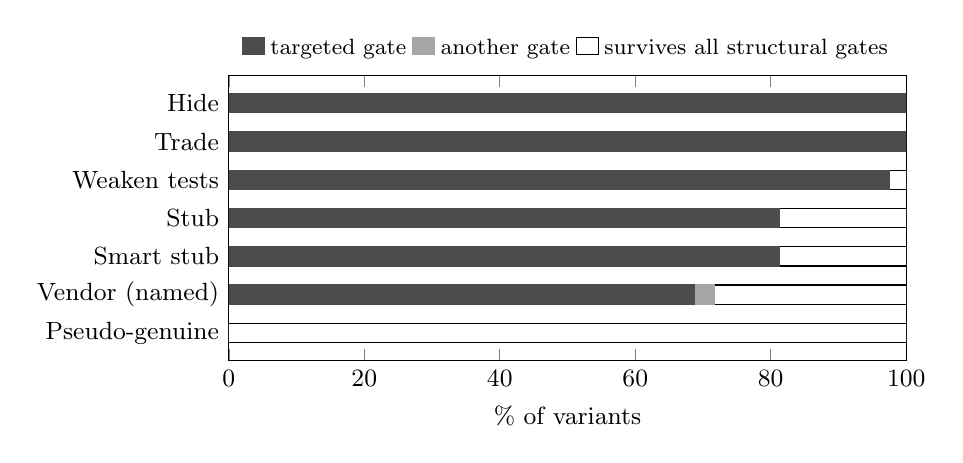
\begin{tikzpicture}
\begin{axis}[
  xbar stacked, width=0.84\columnwidth, height=5.2cm, bar width=7pt,
  xmin=0, xmax=100, xlabel={\% of variants}, xlabel style={font=\small},
  symbolic y coords={{Pseudo-genuine},{Vendor (named)},{Smart stub},Stub,{Weaken tests},Trade,Hide},
  ytick=data, y tick label style={font=\small}, tick label style={font=\small},
  legend style={at={(0.5,1.02)},anchor=south,legend columns=3,font=\footnotesize,draw=none},
  enlarge y limits=0.12]
\addplot[fill=black!70, draw=black!70] coordinates {(100,Hide) (100,Trade) (97.5,{Weaken tests}) (81.3,Stub) (81.3,{Smart stub}) (68.7,{Vendor (named)}) (0,{Pseudo-genuine})};
\addplot[fill=black!35, draw=black!35] coordinates {(0,Hide) (0,Trade) (0,{Weaken tests}) (0,Stub) (0,{Smart stub}) (3.0,{Vendor (named)}) (0,{Pseudo-genuine})};
\addplot[fill=white, draw=black] coordinates {(0,Hide) (0,Trade) (2.5,{Weaken tests}) (18.7,Stub) (18.7,{Smart stub}) (28.3,{Vendor (named)}) (100,{Pseudo-genuine})};
\legend{targeted gate, another gate, survives all structural gates}
\end{axis}
\end{tikzpicture}
\caption{Where each counterfeit is stopped by the structural gates (counts in Appendix~\ref{app:matrix}). Only the pseudo-genuine kind survives every structural gate; \S\ref{sec:rq4} shows where the behavioural gate catches it.}
\label{fig:stopped}
\end{figure}

Figure~\ref{fig:stopped} is the exhibit.
Hidden declarations and trades are stopped completely, test weakening in 78 of 80, stubs and smart stubs with \nStubSurvive{} of 80 surviving the shadow check and the closure gate, and named vendored copies with \nVendorSurvive{} of 67 surviving.
Those survivors are what the tests exist to catch: a stub that shadows nothing returns nothing, and a vendored copy under its own name is the library, so under a conventional grader, without the block, stubs pass CI 8 times in 62 and vendored copies 18 in 52 in the replication corpus, while hidden declarations pass 35 times in 62.
The main corpus was not run through CI, so the figure measures the structural gates as run; the fingerprint check since added to G3 catches \nVendorNamedCaught{} of \nVendorNamed{} named copies and \nVendorRenamedCaught{} of \nVendorRenamed{} copies with every identifier renamed and comments stripped, with no false positive on the references, the pseudo-genuine rewrites, the smart stubs, or the honest deletions.
The pseudo-genuine kind survives every structural gate 80 times in 80: it shadows nothing, copies nothing, touches no test, and shrinks the closure, and the structural checks have nothing left to say.
That is the bridge to RQ4.
The honest-deletion control is rejected once, on a variant whose declaration was in fact still present, which is the correct verdict.
On the \nOverDeclGraded{} over-declared removals, the grader accepts \nFRAccepted, returns inconclusive on \nFRInconclusive{} whose dependency closure it could not resolve, and flags \nFRFlagged: a package moved to an extras group rather than removed.
That flag is correct, and it also means one candidate the attribution called over-declared was not; the attribution's precision is therefore at least that one case short of perfect, and we report it as such.

\subsection{RQ4: Where can the removed library act as the oracle?}
\label{sec:rq4}

\textbf{Where the gate can observe the replacement, every counterfeit rewrite diverges on every generated input and every correct rewrite is accepted; where it cannot, it returns inconclusive, and that boundary, reached while grading these same references, is the result.}

\paragraph{Coverage.}
Recordings exist for \nTracedPairs{} of the \nPairs{} pairs, \nTraceCalls{} calls in all, re-recorded with the current recorder; \fidelityWhole\% of recorded values are compared on the whole value rather than on a representation, against \fidelityWholeBefore\% for the same projects recorded under the earlier summariser, which capped long values instead of hashing them.
For the remaining pairs the recorder loaded but recorded no call (\nRecLoadedNoCall, which is a property of those suites rather than a gap in the method), was not observed loading (\nRecNotObserved), or the suite was not green under it (\nRecNotGreen).
Before the recorder wrote through pytest's saved console descriptor, \nRecNotObservedOld{} pairs were in the second group and \nTracedPairsOld{} were traced; the fix moved almost all of them into the first two.
Coverage, not fidelity, is the binding limit on this gate, and we report it as such.


\begin{table}[t]
\centering
\small
\setlength{\tabcolsep}{4pt}
\begin{tabular}{p{1.75cm}p{2.3cm}p{2.3cm}}
\hline
 & \textbf{Replacement observable} & \textbf{Not observable} \\
\hline
Counterfeit (pseudo-genuine) & \nPseudoEvaluable{} of \nPseudoEvaluable{} rejected, each on \nFuzzInputs{} of \nFuzzInputs{} inputs & \nPseudoOutside{} of \nPseudo{} outside coverage \\
Correct (reference) & \nRefsAccepted{} of \nRefsAccepted{} accepted, 0 rejected & \nRefsInconclusive{} inconclusive, 0 rejected \\
\hline
\end{tabular}
\caption{The behavioural gate's boundary. ``Observable'' means the recorder captured the replacement at the library boundary or at a usage site; ``not observable'' means it captured nothing: the suite recorded no library call locally (\nRefsNoCalls{} references) or the only sites are at module level or in decorators no test exercises (\nRefsNotObservable). Counts are rewrites; the four pseudo-genuine rewrites expose five library functions, all five diverging.}
\label{tab:boundary}
\end{table}

\paragraph{The boundary.}
Table~\ref{tab:boundary} crosses correct against counterfeit with observable against not.
Of the \nPseudo{} pseudo-genuine rewrites, \nPseudoTraced{} fall on a recorded pair and \nPseudoEvaluable{} expose a function the recording shows the repository calling; all \nPseudoEvaluable{} are rejected, each on every one of \nFuzzInputs{} generated inputs, including the running example.
Of the \nRefs{} references, \nRefsEvaluable{} are evaluable in the local run.
The gate accepts \nRefsAccepted: \nRefsNewModuleAccepted{} whose replacement is a new module, reproduced at the library boundary, and one inlined rewrite, reproduced at the usage site where the boundary saw nothing.
It returns inconclusive on \nRefsInconclusive{} and rejects none: \nRefsNoCalls{} suites record no library call on our machine, and \nRefsNotObservable{} use the library only at module level or in a decorator that no test exercises, so there is nothing at either level to compare.
One accepted reference showed 39 usage-level differences, all from a function returning git hashes, which the nondeterminism rule set aside.

\begin{figure}[t]
\centering
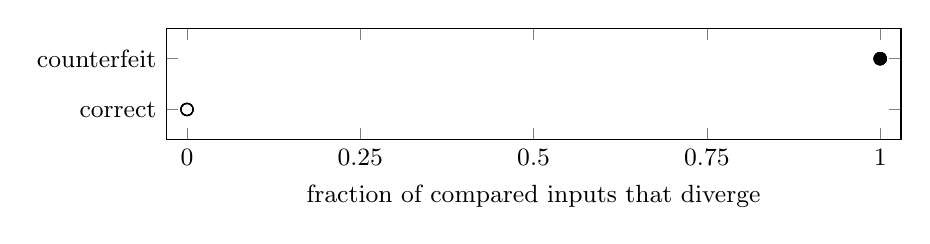
\begin{tikzpicture}
\begin{axis}[width=0.9\columnwidth, height=3.0cm, xmin=-0.03, xmax=1.03, ymin=0.4, ymax=2.6,
  xlabel={fraction of compared inputs that diverge}, xlabel style={font=\small},
  ytick={1,2}, yticklabels={correct, counterfeit}, y tick label style={font=\small},
  tick label style={font=\small}, xtick={0,0.25,0.5,0.75,1}]
\addplot[only marks, mark=*, mark size=2.2pt, black] coordinates {(1,2) (1,2) (1,2) (1,2) (1,2)};
\addplot[only marks, mark=o, mark size=2.2pt, black] coordinates {(0,1) (0,1) (0,1) (0,1) (0,1)};
\end{axis}
\end{tikzpicture}
\caption{Separation where the gate can observe. Counterfeit: five functions from four pseudo-genuine rewrites, each diverging on \nFuzzInputs{} of \nFuzzInputs{} generated inputs. Correct: five references, each agreeing on every recorded input. The inputs differ by row and the counts are small; the margin, not the count, is the evidence.}
\label{fig:separation}
\end{figure}

\paragraph{A development result.}
The \nRefsAccepted{} of \nRefsAccepted{} were reached after four changes to the gate made while grading these same references: pairing by site and order rather than by arguments, equality that ignores a differing type name when the structure is equal, path normalisation, and the usage-site level with its inconclusive rule.
Before them the gate rejected 7 of \nRefsEvaluable.
No reference was held out, so the acceptance figure is a development result, not an evaluation; it shows the gate can accept correct rewrites of this kind, and a held-out set is needed to estimate how often.

\subsection{RQ5: What is in the benchmark, and how do agents do?}
\label{sec:rq5}

\textbf{The pool is \nPairs{} pairs over \nPoolRepos{} repositories, mostly narrow; the task is neither trivial nor impossible, and the grader's verdict on the few CI passes is \todo{pending}.}

\begin{table}[t]
\centering
\small
\begin{tabular}{lrr}
\hline
\textbf{Tier} & \textbf{Pairs} & \textbf{References} \\
\hline
Narrow (1--2 files) & \nTierNarrow{} & \todo{n} \\
Medium (3--4) & \nTierMedium{} & \todo{n} \\
Wide (5+) & \nTierWide{} & \todo{n} \\
Indirect track & \nTierIndirect{} & 0 \\
\hline
Total & \nPairs{} & \nRefs{} \\
\hline
\end{tabular}
\caption{Pool composition and reference coverage. The indirect track is reached through a tool or plugin with no import; \nRefsPass{} of the \nRefs{} references pass the workflow under the block.}
\label{tab:pool}
\end{table}

Table~\ref{tab:pool} gives the composition.
Of \nRefs{} hand-written references, \nRefsPass{} pass the workflow with the package blocked and every structural gate, two of them after a lint fix to the reference's own code (an imperative docstring, a \code{noqa}, and type annotations).
In the pilot, \nAgents{} agents made \nAgentAttempts{} attempts on \nAgentTasks{} pairs and \nAgentPass{} passed the suite, the number a conventional benchmark would report.
\todo{Grader verdicts on the \nAgentPass: rejected by tests or behaviour; rejected on a constraint the prompt did not state (trade, vendor); inconclusive because the pair has no recording. With coverage at \nTracedPairs{} of \nPairs, inconclusive is the likely majority, and the paragraph should say what that means: the grader withholds a verdict it cannot support rather than inheriting the suite's.}

\section{Conclusion}
\todo{Conclusion, to be written after the pending results land.}

\section*{Limitations}
\label{sec:limitations}

\paragraph{The behavioural gate's acceptance is a development result.}
Four changes to the gate were made while grading the same \nRefs{} references that now measure its false rejection, and no reference was held out.
The \nRefsAccepted{} of \nRefsAccepted{} accepted shows that correct rewrites of this kind can be accepted; it does not estimate how often a fresh one would be.
A held-out set, and mutation analysis of the observable references, are the measurements that would.

\paragraph{The gate speaks for a minority of pairs.}
Recordings exist for \nTracedPairs{} of \nPairs{} pairs, and \nRefsInconclusive{} of \nRefsEvaluable{} references are inconclusive because the suite never calls the library on our machine or uses it only at module level.
Where the gate cannot see it says so, and the structural gates and the tests carry the grade; coverage is reported with every verdict.

\paragraph{Thirteen silent runs are set aside, not resolved.}
The activation rule excludes \nExclInconclusive{} silent runs from seven repositories; they were replayed with the corrected block and it never announced itself, so whether their suites are blind or merely never loaded the block is unknown, and the census is reported with and without them.

\paragraph{Winnability is demonstrated for a sample.}
\nRefsPass{} of \nRefs{} hand-written removals pass the workflow under the block, over \nRefsRegular{} regular and \nRefsLarge{} large pairs chosen by the authors, none in the indirect track; for the other pairs admission establishes only that the oracle sees the removal.

\paragraph{The counterfeit corpus was not run through CI.}
The structural results measure what the gates see; whether each variant passes the tests is known only for the replication corpus, and the corpus author also wrote two of the gates.
\todo{State the corpus and reference provenance once the authors confirm it.}

\paragraph{Derived oracles.}
The verdicts of the import check and of collection-only grading are projections onto our population from what each oracle inspects, not runs of those systems; the projection favours the import check.

\paragraph{Open routes.}
Two reflection escapes defeat the block and therefore G5, and a test runner invoked through a Makefile or script lies outside what G7 inspects.
The grader faces an adaptive submitter and is not adversarially complete.

\paragraph{Scope.}
All results are Python, on the repositories of one benchmark, selected for runnable CI, which biases against finding blindness.
The pilot is \nAgentAttempts{} attempts and supports no rate estimate; its gate verdicts are pending.

\section*{Acknowledgments}

\todo{acknowledgments}

% Custom bibliography entries only
\bibliography{custom}

\appendix
\section{Harness Details}
\label{app:harness}
The published \dibench{} harness requires the \code{sysbox} container runtime, which hosted GitHub Actions runners do not provide; we install it in the job, because plain privileged Docker-in-Docker fails when the inner daemon cannot stack overlay filesystems.
In the stability measurement, two replays count as a repeat only if their manifest changes are identical byte for byte; the injected block file is compared separately, because its generator changed between screening generations.
The block is installed through \code{sitecustomize.py} and the root \code{conftest.py}, so it loads in every interpreter the workflow starts in the repository, including subprocesses and multiprocessing workers.
A module that a foreign frame has already loaded is replaced in \code{sys.modules} by a guard that forwards attribute access for foreign callers and raises for repository callers, so import order cannot defeat the block.
Fifteen constructed bypasses were tried against it; thirteen are blocked, including dynamic imports by computed name, \code{exec} strings, subprocess interpreters, re-import after deleting the module entry, and reload.
Two escapes remain open, and a submission could use either on purpose: reaching the real module through \code{object.\_\_getattribute\_\_} on the guard, and listing the module through \code{pkgutil.iter\_modules}.
Neither is reachable by accident; both are recorded because the grader faces an adaptive submitter, and \S\ref{sec:method-grade} states how the grader treats them.




\section{Grader Details}
\label{app:grader}
\paragraph{Summaries and equality.}
Primitives are recorded exactly, strings and bytes past 300 characters with a hash of the whole; containers to depth three with up to 20 elements, beyond which a hash decides; arrays by shape and dtype, with content inlined up to 64 elements and hashed beyond; callables and classes by type and qualified name; other objects by type name, address-stripped representation, length, and public non-callable attributes to depth two.
Floats compare within a relative tolerance of $10^{-9}$ and NaN equals NaN.
A record is bounded at 32\,KB, with expanded structure replaced by its hash beyond that.
\paragraph{Generated inputs.}
A neighbour of a recorded string applies one to a third as many edits as it has characters, each an insertion, deletion, substitution, duplication, or case change; numbers, booleans, and containers are perturbed by type-specific rules, and type-directed values are drawn for breadth.
Inputs are generated from a fixed seed and the first 200 recorded calls per function.
\paragraph{Replication corpus.}
A second corpus of hide, vendor, and stub variants was generated by a separate generator over narrow-tier pairs and run through the CI harness, so it carries G2 verdicts the main corpus lacks.
It overlaps the main corpus on 57 identical (repository, kind, dependency) triples and is never summed with it.



\section{Gate by Kind}
\label{app:matrix}
\begin{table}[h]
\centering
\small
\setlength{\tabcolsep}{3.5pt}
\begin{tabular}{lrrrrrrr}
\hline
\textbf{Kind} & $n$ & G1 & G3 & G7 & G8 & \textbf{Rej.} & Tests \\
\hline
Hide & 77 & \textbf{77} & 0 & 0 & 0 & 77 & 35/62 \\
Trade & 73 & 0 & 0 & 0 & \textbf{73} & 73 & -- \\
Weaken tests & 80 & 0 & 0 & \textbf{78} & 0 & 78 & -- \\
Stub & 80 & 1 & \textbf{65} & 0 & 8 & 65 & 8/62 \\
Smart stub & 80 & 1 & \textbf{65} & 0 & 8 & 65 & -- \\
Vendor (named) & 67 & 1 & \textbf{46} & 0 & 14 & 48 & 18/52 \\
Pseudo-genuine & 80 & 0 & 0 & 0 & 0 & \textbf{0} & -- \\
\hline
Honest deletion & \nHonest{} & 1 & 0 & 0 & 1 & 1 & -- \\
Over-declared removal & \nOverDeclGraded{} & 1 & 0 & 0 & 0 & 1 & \nOverDeclGraded{} \\
\hline
\end{tabular}
\caption{Structural gates over the constructed variants. Cells count variants the gate rejects; bold marks the gate each kind targets; ``Rej.'' counts variants any gate rejects. ``Tests'' is the share passing CI, available from the replication corpus for three kinds (its $n$ differs) and by construction for the over-declared removals; the main corpus was not run through CI. Rows below the rule are controls that must pass.}
\label{tab:matrix}
\end{table}
\section{Robustness of the Silent Rate}
\label{app:robustness}
Over the \nReposThree{} repositories with at least three candidates, after the activation rule; figures with the \nExclInconclusive{} set-aside runs counted in parentheses.

\begin{center}\small
\begin{tabular}{lrrr}
\hline
Dropped & Repositories & Median & Incidence \\
\hline
0 & 49 (51) & 18.8\% (20.0) & 33/49 (35/51) \\
1 & 48 (50) & 17.7\% (20.0) & 32/48 (34/50) \\
3 & 46 (48) & 15.5\% (19.4) & 30/46 (32/48) \\
5 & 44 (46) & 14.3\% (17.7) & 28/44 (30/46) \\
10 & 39 (41) & 12.5\% (14.3) & 23/39 (25/41) \\
\hline
\end{tabular}
\end{center}

Distribution of the rate: 0\%: 16; 1--10\%: 1; 10--25\%: 14; 25--50\%: 13; over 50\%: 5.
Correlation of the rate with the share of files that are tests, $-0.30$; with the share reachable from tests, $-0.36$; with the number of candidates, $+0.37$.
Repositories maintained by large organisations with at least one silent candidate: cowrie 8 of 10, NVFlare 5 of 18, localstack 6 of 15, nncf 6 of 17, chalice 3 of 10, docker-py 1 of 3, dm-haiku 1 of 4, mobly 1 of 3, jupyter-console 1 of 8; speakeasy 0 of 6, and tweepy 0 of 1 once its two silent candidates are set aside by the activation rule.

\section{Oracle Overlap}
\label{app:overlap}
Per candidate, over the \nScreenedRule{} candidates not excluded. CI is measured; the other two are derived (\S\ref{sec:derived}).

\begin{center}\small
\begin{tabular}{llll r}
\hline
CI & Import check & Collection-only & & $n$ \\
\hline
detects & detects & detects & & 223 \\
detects & detects & silent & & 75 \\
detects & silent & detects & & 24 \\
detects & silent & silent & & 8 \\
silent & detects & silent & strict blindness & \nImportCatchesCIMisses{} \\
silent & silent & silent & & 183 \\
\hline
\end{tabular}
\end{center}

\end{document}
